

\chapter{Progress} 

A Medical Bsc student used linear normalisation, global histogram equalisation and contrast limited adaptive histogram equalisation to enhance image, and the videos were processed through eularian colour magnification. The findings in that report have confirmed that image processing can be used to improve image contrast and subsequently aid in the detection of erythema. This applies to all skin colours \cite{Mohammed}.\\

This report will using his findings and test more image process algorithms and implement them to the software. In the meantime, using MATLAB image process toolbox to test the algorithm is necessary to implement them to the software quickly.\\

Due to the skin color diversity, it requires multiple algorithm for different skins and individuals. Skin colors are important for a broad range of imaging applications to assure quality and naturalness. This report will discuss the impact of various metadata on skin colors in images. The software will be implemented by the
refined skin color models from framework improve the accuracy of skin detection.\\

Besides, except image process tools implemented in the software, it also includes basic image draw tools as a windows desktop application to improve the user interaction, such as:
\begin{itemize}
\item File: Open an image, Save, and Exit.
\item Editor: Undo, Redo, Copy, Paster, Reset ( Reset the image to the original One)
\item View: Initial Size, Zoom In, Zoom Out, Fit to Screen, Right Rotate, Left Rotate
\item Adjustments: The image enhancement is in the Adjustments tools part
\item Help: Helper, and About PUimage
\end{itemize}

\section{Overview of Project}

Basically, the pressure ulcer image processing software works as followed: 
\begin{itemize}
\item Medical staff create an accountant in the database of PUimage software, and login to initial some basic settings;
\item The user (medical staff) get the patients' skin image data in some frequency (like per week, depending on patients' situation), upload to the software;
\item Using Image adjustment tools to analyse the image, store results in the database;
\item Update the skins' evaluation diagram. It is useful to monitor the patients' evalution;
\item Until the pressure sore of the patient is reversed.
\end{itemize}
The software is described in Figure 3.1.
\begin{figure}
	\centering
	\includegraphics[scale=0.6]{ProjectD}
	\caption{Project Activity Diagram}
\end{figure}

\section{Specifications} 
Main high level essential requirements of the software proposed by the professor include the creation of a component, that is responsible for analyze the skin images, as well as the medical staff and patients database. Table 1 demonstrates the low level specifications derived from the aforementioned requirements by applying the simplified version of van Lamsweerde\textquotesingle s KAOS goal-oriented model, questioning how and why a particular requirement is applied. Table 3.1 is grouped by a particular component of the software and includes a relevant risk levels.\\
\subsection{Requirements}
\subsubsection{External interface Requirements}
\begin{itemize}
\item{User interfaces}
A first-time user of the mobile application should see the log-in page when he/she opens the application. If the user has not registered, he/she should be able to do that on the log-in page. Every user should have a profile page where they can edit their e-mail address, phone number and password, and their patients' database.
\item{Software interfaces}
The mobile communicates with the mobile phone in order to get image information
, and with the database in order to get the information about the user and hospital location and related information.
\end{itemize}
\subsubsection{Functional Requirements}
Details are updated the table.
\subsubsection{Performance requirements}
The requirements in this section provide a detailed specification of the user interaction with the software and measurements placed on the system performance. 
\begin{itemize}
\item{Image Process Algorithm Performance}
Efficient multiple image processing is based on data training performance.
\item{Application memory} 
 The amount of Operate System memory occupied by the application
\item{Software Availability and Internet Availability}  The availability of the system when it is used and connecting to the Internet.
\item{Security} If an admin tries to log in to the web portal with a non-existing account then the admin should not be logged in. The admin should be notified about log-in failure
\begin{center}
\captionof{table}{Specifications Table} \label{tab:title2} 
\begin{tabular}{ | m{4.5cm}| m{9cm} | m{1cm} |} 
\hline
Component & Description & Risk\\ 
\hline
User Login & Creating an interface to Login into the system & L \\ 
\hline
User Input Info & Creating a user interface that allows the user to input the
users' information as well as his or her patients' related information& L \\ 
\hline
Windows applicaitons Function & File: Open an image, Save, and Exit & L \\
\hline
Windows Image Editor & Editor: Undo, Redo, Copy, Paster, Reset ( Reset the image to the original One) & L \\
\hline
Windows Image Viewer & Initial Size, Zoom In, Zoom Out, Fit to Screen, Right Rotate, Left Rotate & L \\
\hline
Image Adjustment Tools & Implement multiply image processing algorithms and user choose suitable parameter for different individuals & L \\
\hline
Image Difference Evaluation Diagram & Create a patients treatment changes based on the timeline & L \\
\hline
Database & Development of a database in place of hash table storing relevant
data & L \\
\hline
Software Support & Extension of the software to support multiple computer system and exploring the possibility of support on mobile devices & H \\
\hline
\end{tabular}
\end{center}

\section{Plan}
I have already broken the project down into three main parts: modelling, implementation and evaluation. Modelling will focus on image process algorithms. In the implementation phase, the model is transformed in computer code and implemented into the software. During modelling and implementation are sufficiently far along that the code is producing results, then the evaluation stage can begin and results can be
analysed. Although separate they are not independent. For example, difficulties in implementation may require a rethink in the model, the implementation must include code that stores results for evaluation and evaluation of results may lead to changes in the model. Most of the progress so far has been on modelling and so I shall focus on it for this chapter.
\subsection{Methodology}
\subsubsection{System Boundaries}

Main components of the programs will be developed using C++ language. The reasoning behind such is Dlib, which is a modern C++ toolkit containing machine learning algorithms and tools for creating complex software in C++ to solve real world problems\cite{dlib}. Moreover, C++ with OpenCV library is usually popular for performance critical image processing applications. Written in optimized C++, the library can take advantage of multi-core processing \cite{opencv}.\\

The possible challenge that could arise is the lack of previous experience in Image Process, as well as a number of solutions that could be adopted to develop a complicated analysis and management system. To ensure the refactoring of the code is kept to minimum, thorough research of the languages and available tools will be conducted prior any development takes place.

\subsubsection{Development Techniques}

Due to schedule constraints and lack of previous development experience, the development
process will take place iteratively \cite{Change}. Such approach allows for creation of mini-projects, which appears to be less risky than a spiral model in the instance where additional features would not be possible to implement.\\

Moreover, the project will be adopting the Agile ideology \cite{Sutherland} with Scrum framework, because of more flexible model of Scrum over XP, and a greater suitability for smaller, as in this instance, development teams. As far as the version control system is concerned, the distributed approach as opposed to centralized will be adopted due to the flexibility it offers and the option to work on several features
simultaneously. Although it is believed that distributed model could be more difficult to maintain and prone to merge conflicts \cite{Hardeep}, previous experience with the Git-based software, along with daily meetings should reduce such risks to minimum. Moreover, the project repository will be hosted at the Github, providing with
an opportunity of immediate support in case of unexpected issues with the system.


\subsection{Implementation}
The process of implementing the image process methods into computer code must be broken down into smaller tasks. This will also include basic windows menu design, image adjustment methods, database setting, are appropriate to use. This project is more than producing a software but I consider it as a significant portion to be software engineering.  As such I will layout briefly how I plan to follow good practices. 

\subsubsection{Image Process Algorithm}
The software will provide a comprehensive set of reference-standard functions for image processing, analysis, visualization, and algorithm development. The user can perform image analysis, image enhancement, noise reduction, geometric transformations, and image registration. 

\subsubsection{Version Control}
I will keep my code (including all the reports) under version control using Git. Git is very useful to use on individual projects since it does not require setting up a server for repositories unlike centralized version control systems such as Subversion. Using Git also allows me to backup my code on Github where anyone can follow my progress if they want, \url{https://github.com/Shanshan-IC/MscProject}. 
For instance the source for this Latex document can be found at \url{https://github.com/Shanshan-IC/MscProject/Backgroundreport}.

\subsubsection{MATLAB}
The software will be implemented image processing algorithms based on data test results on MATLAB image process toolbox.

\subsubsection{OpenCV}
The software will be developed by Visual Studio 2012 with OpenCV. OpenCV (Open Source Computer Vision Library) is an open source computer vision and machine learning software library. OpenCV was built to provide a common infrastructure for computer vision applications and to accelerate the use of machine perception in the commercial products.

\subsubsection{Database}
In the middle of stage, the software will be implemented the database to help nurses and doctors to store patients' skin analysis data and monitor the progress during the detection stage.

\subsubsection{Test Driven Developement}
Test-driven development is an advanced technique that uses unit tests to drive the design of software. The suite of unit tests provides constant feedback that each component is still working and act as documentation that cannot go out-of-date.


\subsection{Evaluation}
In order to evaluate all the image process methods, it is necessary to decide
first what should be considered as successful outcomes and then how
these should be measured. For example, different images taken from nurses gains better effect results using different algorithm and why, and as a whole, which might be
measured as the best solution for analysis, setting it as default.

\subsection{Proposed Schedule}
Due to selected iterative model, the scheduling strategy consists of the division of the project development into one research phase and four goal-oriented phases \cite{Hardeep}. Each phase is inclusive of the technical group meeting for the ticketing purposes, as well as the ongoing testing and documentation. Moreover, a follow-up meeting with the professor will take place after the completion of each phase to ensure all the requirements were met as expected.\\

\graphicspath{Timeline}
	\centering
	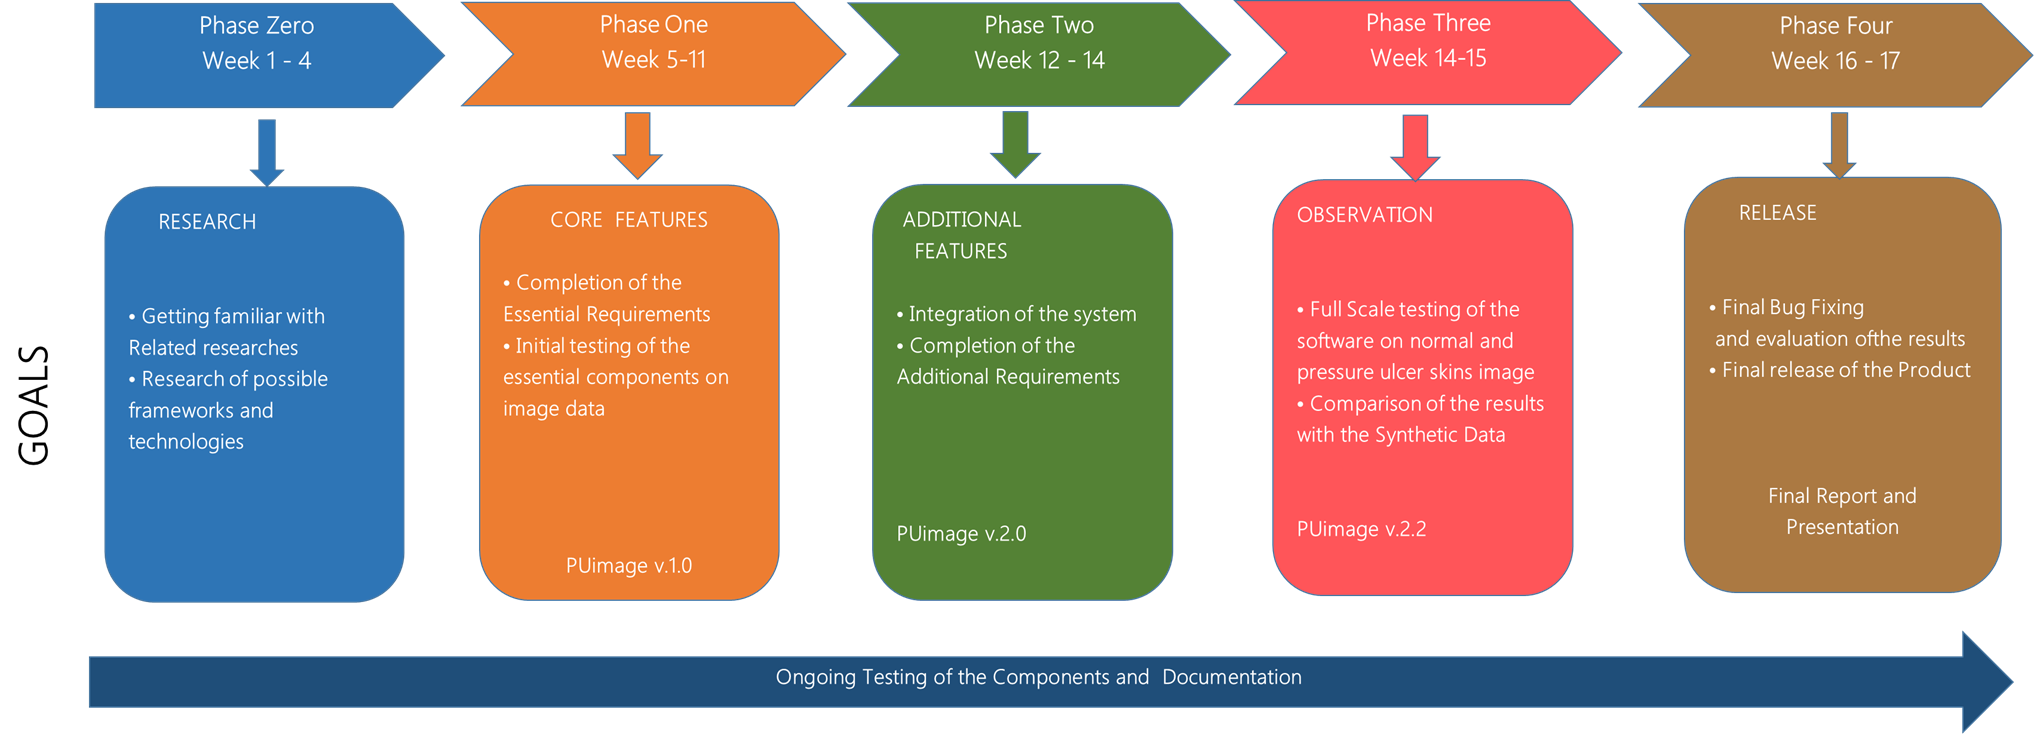
\includegraphics[scale=0.45]{Timeline}
	\caption{Timeline}
\end{figure}
The proposed schedule may be subject to possible changes based on the outcome of the meetings or general alterations of requirements. \\